\begin{frame}{Trilateral Flash Closed Cycle (TFC)}
\begin{columns}
    \column{0.45\textwidth}
    \begin{figure}[h]
      \centering
      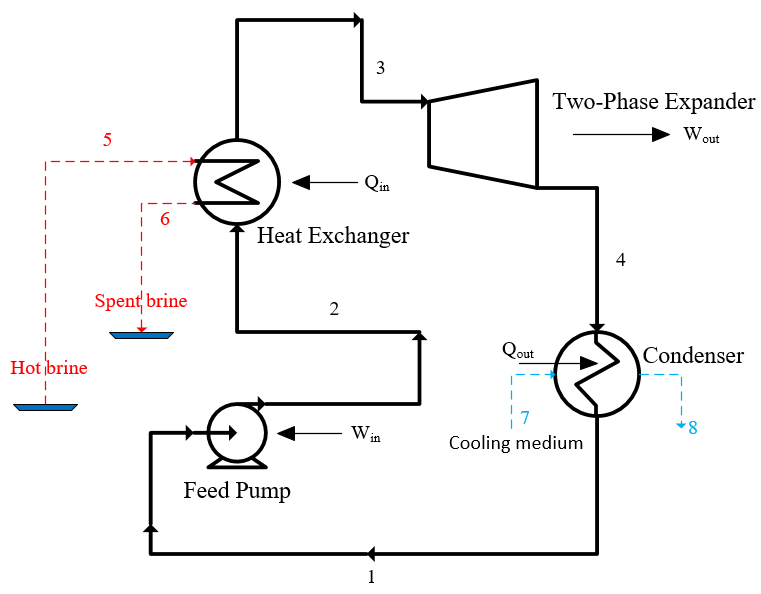
\includegraphics[height=4cm]{images/TLC.png}
      \caption{\scriptsize Schematic Diagram of an Actual Trilateral Closed Cycle (TFC) \cite{smith2014power}}
      \label{fig:tlcschematicdiagram}
   \end{figure}
   \column{0.45\textwidth}
    \begin{figure}[h]
    \centering
    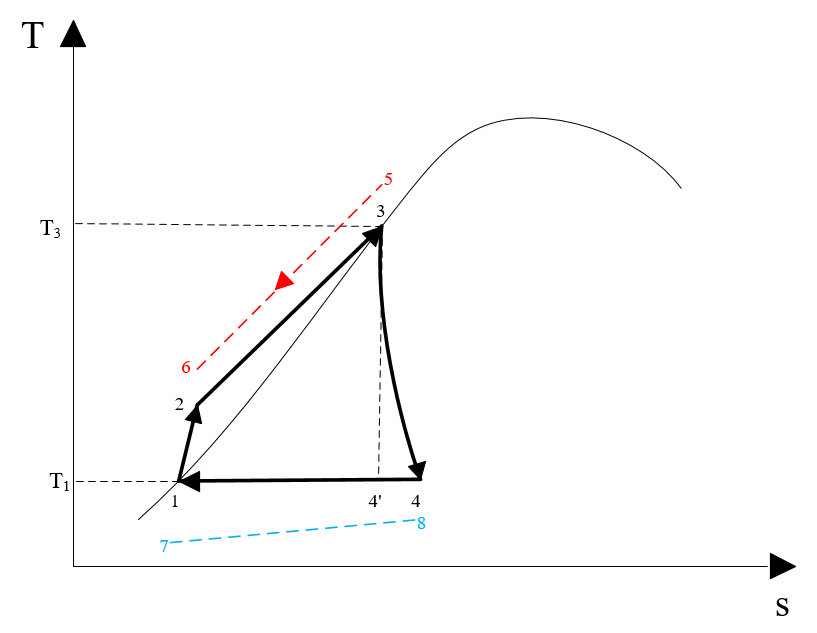
\includegraphics[height=4cm]{images/tfctsdiagram.png}
    \caption{\scriptsize Temperature (T) versus specific entropy (s) diagram of TFC \cite{smith2014power}}
    \label{fig:tlctsdiagram}
    \end{figure}
\end{columns}
\end{frame}

\begin{frame}{Trilateral Flash Closed Cycle (TFC) in NOHTFPECGPPIE}
\begin{columns}
    \column{0.45\textwidth}
    \begin{figure}[h]
      \centering
      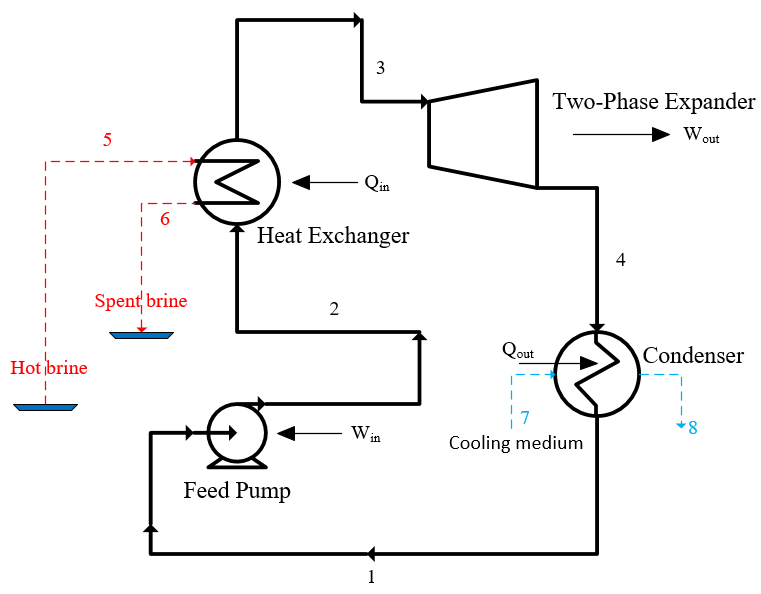
\includegraphics[height=4cm]{images/TLC.png}
      \caption{\scriptsize Schematic Diagram of an Actual Trilateral Closed Cycle (TFC) \cite{smith2014power}}
   \end{figure}
   \column{0.45\textwidth}
    \begin{figure}[h]
    \centering
    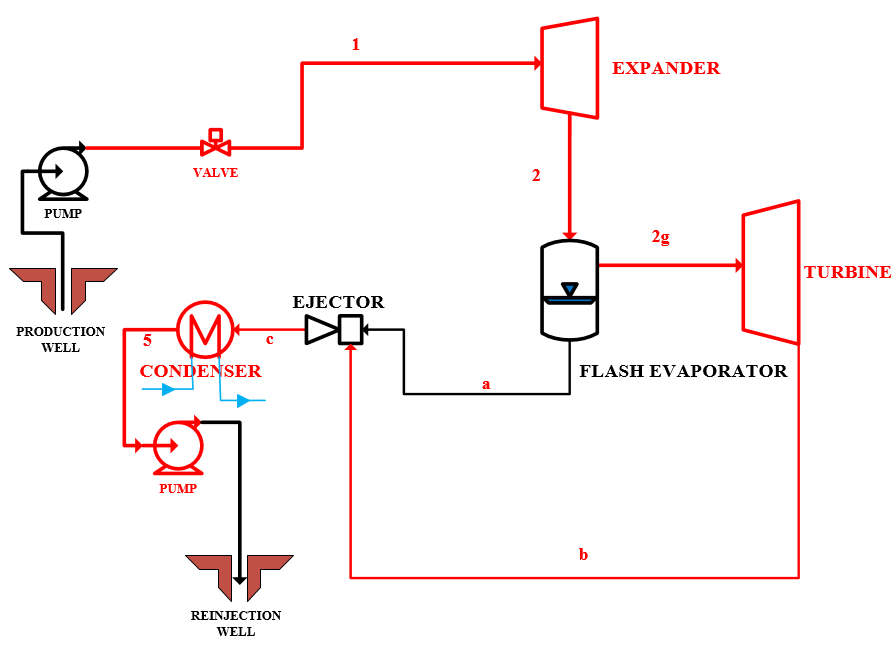
\includegraphics[height=4cm]{images/nohtfpecgppietfc1.png}
    \caption{\scriptsize NOHTFPECGPPIE emphasizing the TFC}
    \end{figure}
\end{columns}
\end{frame}

\begin{frame}{TFC versus BORC}
\begin{columns}
    \column{0.45\textwidth}
    \begin{figure}[h]
      \centering
      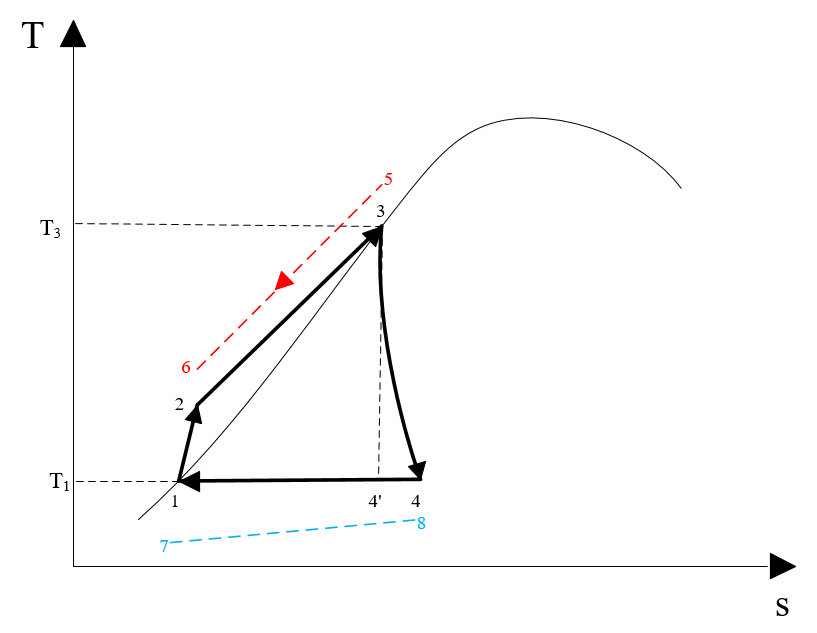
\includegraphics[height=4cm]{images/tfctsdiagram.png}
      \caption{\scriptsize \centering Temperature (T) versus specific entropy (s) diagram of TFC \cite{smith2014power}}
   \end{figure}
   \column{0.45\textwidth}
    \begin{figure}[h]
    \centering
    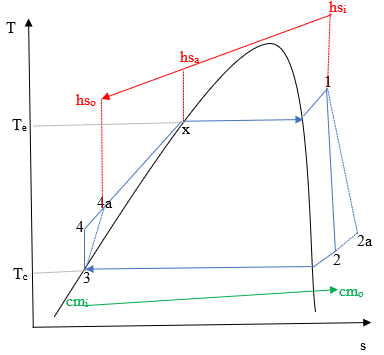
\includegraphics[height=4cm]{images/borctsdiagram.png}
    \caption{\scriptsize \centering Temperature (T) versus specific entropy (s) diagram of Basic Organic Rankine Cycle (BORC)}
    \end{figure}
\end{columns}
\end{frame}

\begin{frame}{TFC versus NOHTFPECGGIE}
\begin{columns}
    \column{0.45\textwidth}
    \begin{figure}[h]
      \centering
      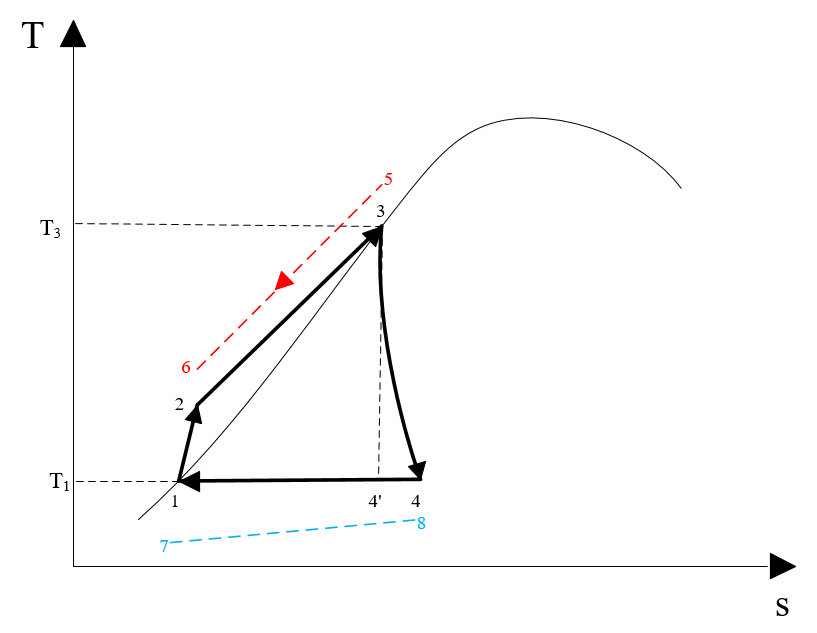
\includegraphics[height=4cm]{images/tfctsdiagram.png}
      \caption{\scriptsize \centering Temperature (T) versus specific entropy (s) diagram of TFC \cite{smith2014power}}
   \end{figure}
   \column{0.45\textwidth}
    \begin{figure}[h]
    \centering
    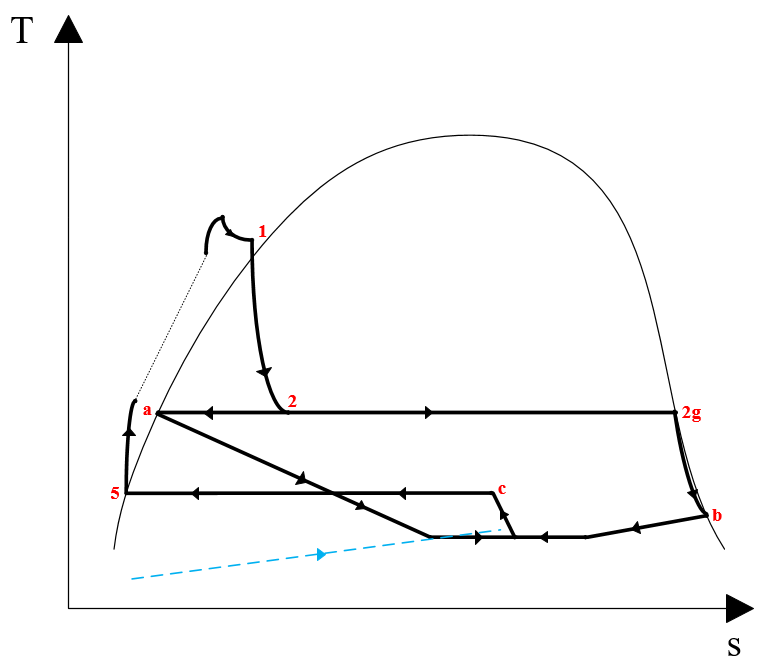
\includegraphics[height=4cm]{images/nohtfpecgppietsdiagram1.png}
    \caption{\scriptsize \centering Temperature (T) versus specific entropy (s) diagram of NOHTFPECGPPIE}
    \end{figure}
\end{columns}
\end{frame}

\begin{frame}{Trilateral Flash Closed Cycle (TFC) Literature}
    \begin{block}{Fischer et al. 2011 \cite{fischer2011comparison}}
    \begin{itemize}
        \item Pros: \textbf{Exergy Efficiency for power production} is \textbf{larger by 14\%-29\%} for the \textbf{Optimized TFC than for the Optimized Organic Rankine Cycle (BORC)} five pairs of temperature ranges.
        \item Cons: TFC has \textbf{Large Volume Expansion Ratios at the Expander} that ranges from \textbf{700-5500} given five pairs of temperature ranges.
        \item Analysis: Thermodynamic Comparative Analysis between TFC and BORC.
        \item  Working Fluid: Water for TFC and Pure Organic Fluid for BORC
        \item Temperature Range: Five pair cases of Evaporating and Condensing Temperatures: (350$^\circ$C,62$^\circ$C), (280$^\circ$C,62$^\circ$C), (280$^\circ$C,15$^\circ$C), (220$^\circ$C,15$^\circ$C) and (150$^\circ$C,15$^\circ$C).
    \end{itemize}
    \end{block}
\end{frame}

\begin{frame}{Trilateral Flash Closed Cycle Literature}
    \begin{block}{Ajimotokan et al. 2014\cite{ajimotokan2014trilateral}}
     \begin{itemize}
         \item Findings: \textbf{30\% to 40\% improvement of thermal efficiency over Organic Rankine} having an Exergy Efficiency of 81.1\%.
         \item Analysis: Thermodynamic Analysis
         \item Working Fluid: Isobutane
         \item Temperature Range: 363-393 K
     \end{itemize}
    \end{block}
\end{frame}

\begin{frame}{Trilateral Flash Closed Cycle Literature}
    \begin{block}{Ajimotokan and Sher (2015)\cite{ajimotokan2015thermodynamic}}
    \begin{itemize}
        \item Findings:
     \begin{table}[h]
         \centering
         \begin{tabular}{cc}
         \hline
             Types of Trilateral Cycles & Thermal Efficiency Range \\
        \hline
              Simple & 11.85-21.97\% \\
              Recuperated & 12.32-23.91\% \\
              Reheat & 11.86-22.07\% \\
              Regenerative & 12.01-22.9\% \\
        \hline
         \end{tabular}
     \end{table}
         \item Working Fluid: N-pentane
         \item Analysis: Thermodynamic Analysis
         \item Temperature Range: 393-443 K
     \end{itemize}
    \end{block}
\end{frame}

\begin{frame}{Trilateral Flash Closed Cycle Literature}
    \begin{block}{Bianchi et al. 2017\cite{bianchi2017numerical}}
     \begin{itemize}
         \item Remarks: Development of a Plug and Play or Packaged type Trilateral Flash Cycle system
         \item Findings: Expected recovered power is 120 kWe and a thermal efficiency of 6\%.
         \item Working Fluid: R1233zd(E) and R245fa
         \item Analysis: Thermodynamic Analysis
     \end{itemize}
    \end{block}
\end{frame}

\begin{frame}{Trilateral Flash Closed Cycle Literature}
    \begin{block}{Li et al. 2017\cite{li2017comparison}}
     \begin{itemize}
         \item Pros: Trilateral Flash Cycle obtains a \textbf{maximum thermal efficiency} of \textbf{14.8\%} at an evaporation temperature of 153$^\circ$C, which is \textbf{40\% higher than that Organic Rankine Cycle} (10.6\%) and \textbf{57\% higher than that of Organic Flash Cycle}. Thermal efficiency of TFC becomes larger than BORC when the evaporation temperature exceeds by 130$^\circ$C.
         \item Cons: It has the \textbf{largest UA value} ranging from \textbf{7.9 kW/$^\circ$C to 8.8 kW/$^\circ$C} for \textbf{evaporation temperatures} of \textbf{100$^\circ$C} to \textbf{150$^\circ$C}, respectively.
         \item Analysis: Thermodynamic Analysis
         \item Working Fluid: R245fa
     \end{itemize}
    \end{block}
\end{frame}

\begin{frame}{Trilateral Flash Closed Cycle Literature}
    \begin{block}{Li et al. 2019\cite{li2019analysis}}
     \begin{itemize}
         \item Remarks: Toluene has the best performance at high-temperature evaporator of 530 K and low-temperature evaporator of 373 K having a maximum power output of 11.3 kW, thermal efficiency of 24.2\% and exergy efficiency of 63.2\%.
         \item Cycle: Combined TLC-ORC
         \item Analysis: Thermodynamic Analysis
         \item Working Fluid for ORC (High Temperature Cycle): Choice of Cyclohexane, Toluene, Benzene and Water
         \item Working Fluid for TLC (Low Temperature Cycle): R245fa
     \end{itemize}
    \end{block}
\end{frame}

\begin{frame}{Trilateral Flash Closed Cycle Literature}
    \begin{block}{Iqbal et al. 2019 \cite{iqbal2019trilateral}}
     \begin{itemize}
         \item Remarks: 
         \begin{enumerate}
             \item TFC has the capability of about \textbf{140\% more power generation than ORC} for the same heat source and sink temperatures.
             \item TFC can be utilized up to \textbf{70\% of available thermal energy} where ORC can only deal with 20\%.
             \item TFC \textbf{allows the heat carrier to leave the system very close to ambient temperature that contribute almost zero to global warming}.
             \item TFC incorporate \textbf{high pumping power} and \textbf{larger heat exchanger and condenser which increases the cost of construction} though it can be compensated by high power generation.
         \end{enumerate}
         \item Analysis: Thermodynamic Analysis, Working Fluid: R1233zd(E)
         \item Heat Source Temperature: 80$^\circ$C, Heat Sink Temperature: Ambient Temperature
     \end{itemize}
    \end{block}
\end{frame}

\begin{frame}{Partial Evaporation Cycles}
\begin{columns}
    \column{0.45\textwidth}
    \begin{figure}[h]
      \centering
      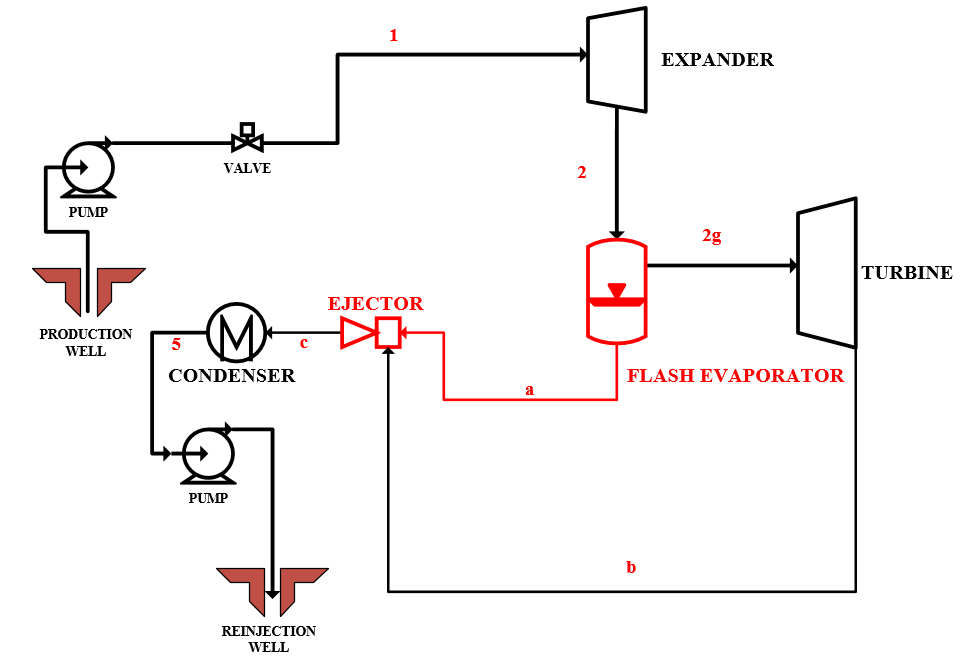
\includegraphics[height=4cm]{images/nohtfpecgppiepe.png}
      \caption{\scriptsize Schematic Diagram of NOHTFPECGPPIE emphasizing the Partial Evaporation}
   \end{figure}
   \column{0.45\textwidth}
    \begin{figure}[h]
    \centering
    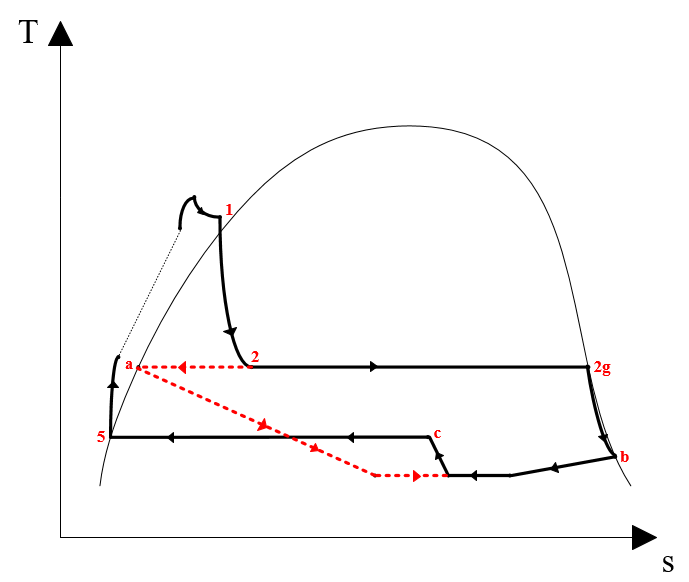
\includegraphics[height=4cm]{images/nohtfpecgppietsdiagram2.png}
    \caption{\scriptsize Temperature (T) versus specific entropy (s) of the NOHTFPECGPPIE}
    \end{figure}
\end{columns}
\end{frame}

\begin{frame}{Effect of the Quality (X) of the Motive Fluid (i.e. at state point a) to the Entrainment Ratio ($\mu$)\cite{wang2016experimental}}
\begin{columns}
    \column{0.45\textwidth}
    \begin{figure}[h]
      \centering
      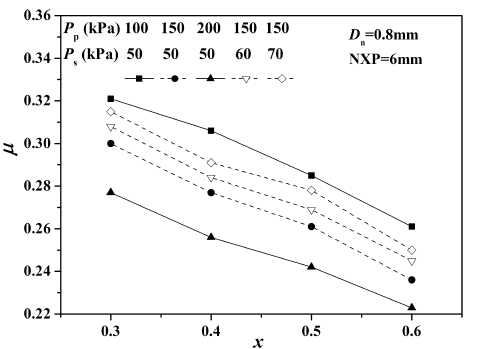
\includegraphics[height=4cm]{images/partialevapmu.png}
      \caption{\scriptsize \centering Effect of the quality (x) to the entrainment ratio ($\mu$) by Wang and Yu (2016) \cite{wang2016experimental}}
   \end{figure}
   \column{0.45\textwidth}
    \begin{block}{Reference}
     Experimental Investigation on two-phase driven ejector performance in a novel ejector enhanced refrigeration system by Wang and Yu 2016 \cite{wang2016experimental}
    \end{block}
    \begin{block}{Entrainment Ratio ($\mu$), Quality (x)}
     $\mu = \frac{\Dot m_{s}}{\Dot m_{p}}$, \: $x = \frac{Volume\:of\:the\:vapor}{Total\:volume\:of \:the\:mixture}$
    \end{block}
\end{columns}
\end{frame}

\begin{frame}{Effect of the Quality (X) of the Motive Fluid (i.e. at state point a) to the Pressure Ratio ($r_{p}$)\cite{wang2016experimental}}
\begin{columns}
    \column{0.45\textwidth}
    \begin{figure}[h]
      \centering
      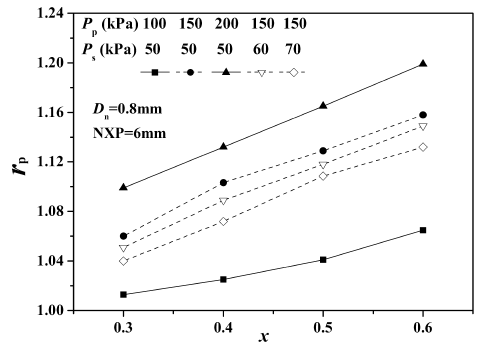
\includegraphics[height=4cm]{images/partialevaprp.png}
      \caption{\scriptsize \centering Effect of the quality (x) to the pressure ratio ($r_{p}$) by Wang and Yu (2016) \cite{wang2016experimental}}
   \end{figure}
   \column{0.45\textwidth}
    \begin{block}{Reference}
     Experimental Investigation on two-phase driven ejector performance in a novel ejector enhanced refrigeration system by Wang and Yu 2016 \cite{wang2016experimental}
    \end{block}
    \begin{block}{Pressure Ratio ($r_{p}$), Quality (x)}
     $r_{p} = \frac{P_{d}}{P_{s}}$, \: $x = \frac{Volume\:of\:the\:vapor}{Total\:volume\:of \:the\:mixture}$
    \end{block}
\end{columns}
\end{frame}

\begin{frame}{Effect of the Quality (X) of the Motive Fluid (i.e. at state point a) to the Ejector Efficiency ($\eta$) \cite{wang2016experimental}}
\begin{columns}
    \column{0.45\textwidth}
    \begin{figure}[h]
      \centering
      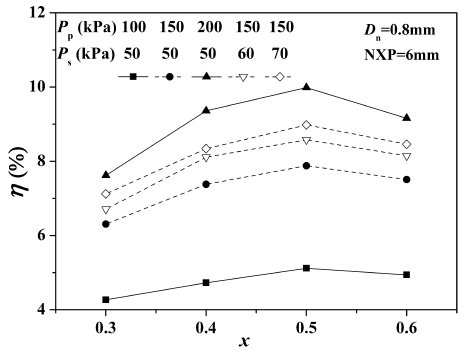
\includegraphics[height=4cm]{images/partialevapejeceff.png}
      \caption{\scriptsize \centering Effect of the quality (x) to the ejector efficiency ($\eta$) by Wang and Yu (2016) \cite{wang2016experimental}}
   \end{figure}
   \column{0.45\textwidth}
    \begin{block}{Ejector Efficiency ($\eta$)}
    Ratio of the actual expansion work recovered by the the ejector $(\Dot W_{rec})$ to the maximum possible work rate recovery $(\Dot W_{rec,max})$
        \begin{equation}
            \eta = \frac{\Dot W_{rec}}{\Dot W_{rec,max}} = \frac{\Dot m_{s}(h_{d}-h_{s})}{\Dot m_{p}(h_{p}-h_{d})}
        \end{equation}
    \end{block}
\end{columns}
\end{frame}

\begin{frame}{Ejector}
\begin{columns}
  \column{0.45\textwidth}
  \begin{block}{Ejector}
   Tashtoush et al.\cite{tashtoush2019comprehensive} defines Ejector as a flow device with two intake ports and one discharge that allows the primary high-pressure stream to entrain the secondary low-pressure stream, where both streams are being mixed inside the ejector and discharged at some intermediate pressure termed as backpressure.
  \end{block}
  \column{0.45\textwidth}
  \begin{figure}[h]
   \centering
   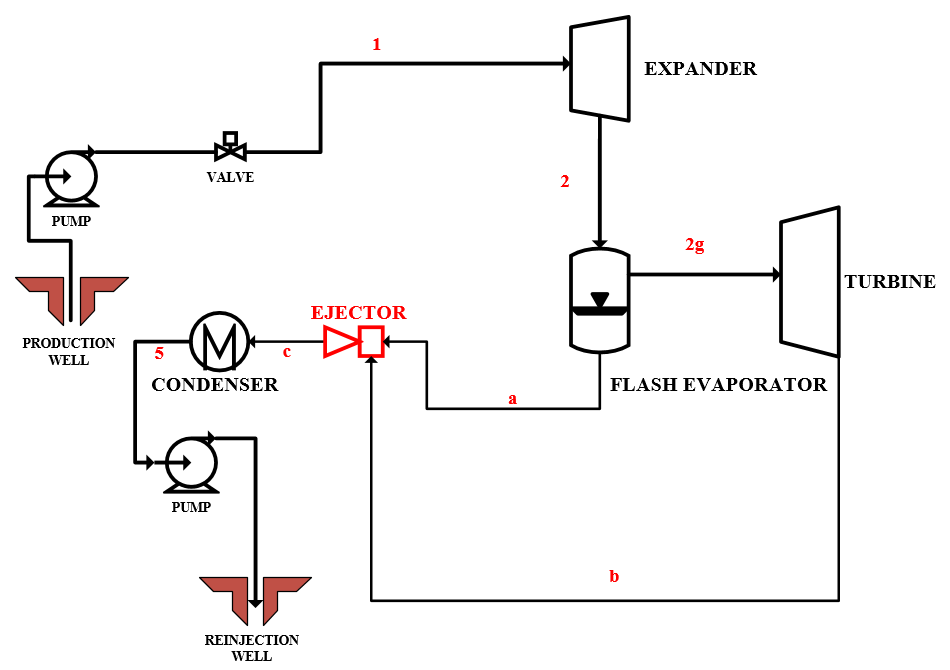
\includegraphics[height=4cm]{images/nohtfpecgppieejector.png}
   \caption{Emphasizing Ejector in NOHTFPECGPPIE}
  \end{figure}
  \end{columns}
\end{frame}

\begin{frame}{Basic Parts of an Ejector drawn using ANSYS R18.0}
  \begin{figure}[h]
    \centering
   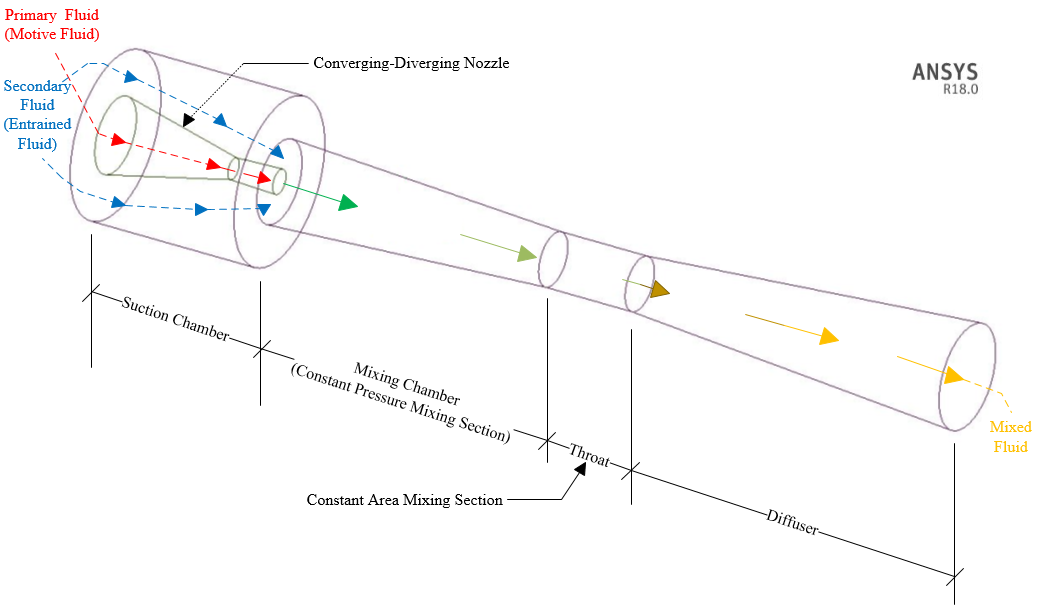
\includegraphics[height=5.25cm]{images/Ejector basic parts.PNG}
    \label{fig:ejectorparts}
  \end{figure}  
\end{frame}

\begin{frame}{Rationale of the Construction of the Ejector}
    \begin{block}{Tashtoush et al. \cite{tashtoush2019comprehensive}}
     Moving the converging-diverging nozzle discharge port away from the ejector's throat (upstream the entrance) would enhance the performance of the ejector by augmenting the entrainment ratio.
    \end{block}
    \begin{block}{Definition of Entrainment Ratio}
     Entrainment Ratio is defined as the ratio of the secondary mass flow rate to the primary mass flow rate. 
    \end{block}
\end{frame}

\begin{frame}{Rationale of the Construction of the Ejector}
    \begin{block}{Pianthong et al.\cite{pianthong2007investigation}}
     The enhancement of the entrainment ratio is occurred when the nozzle exit was positioned away from the ejector throat.\textbf{Positioning the nozzle exit away from the ejector throat increases the effective area of the hypothetical throat between the jet core (steam jet) and ejector wall (mixing nozzle) at which the secondary was entrained before mixing occurred.}
    \end{block}
    \begin{figure}
        \centering
        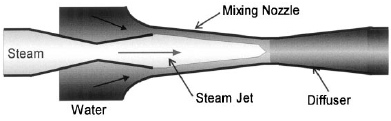
\includegraphics[height=2cm]{images/Central steam jet.PNG}
        \caption{\small Central Steam Jet Ejector based on the illustration of Narabayashi et al. \cite{narabayashi1997study,narabayashi2000study}}
        \label{fig:centralsteamjet}
    \end{figure}
\end{frame}

\begin{frame}{Rationale of the Construction of the Ejector}
    \begin{block}{Chunnanond and Aphornratana\cite{chunnanond2004experimental}}
     When the NXP is moved away from the ejector throat, the expansion waves of the jet core stream would face stronger compression effect and, consequently, smaller expansion angle and larger effective area would be produced.
    \end{block}
\end{frame}

\begin{frame}{Ejectors: Operating Principles}
    \begin{columns}
    \column{0.45\textwidth}
    \begin{figure}[h]
      \centering
      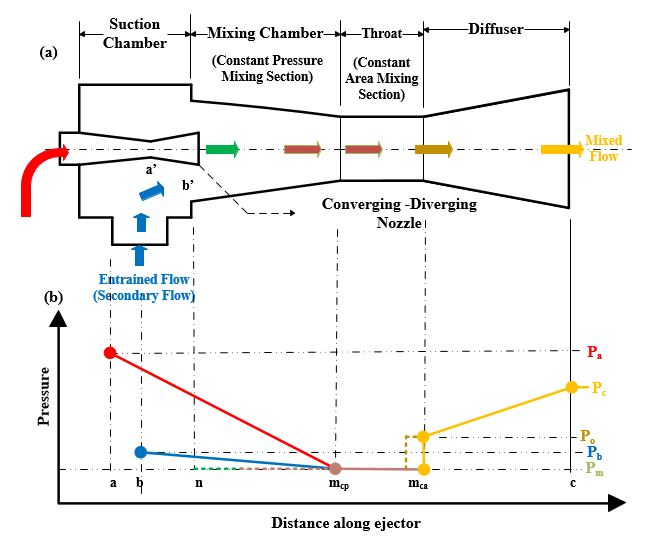
\includegraphics[height=4cm]{images/Ejectorpressureprofile1.JPG}
      \caption{\scriptsize Pressure Profile versus distance along ejector}
   \end{figure}
   \column{0.45\textwidth}
    \begin{figure}[h]
    \centering
    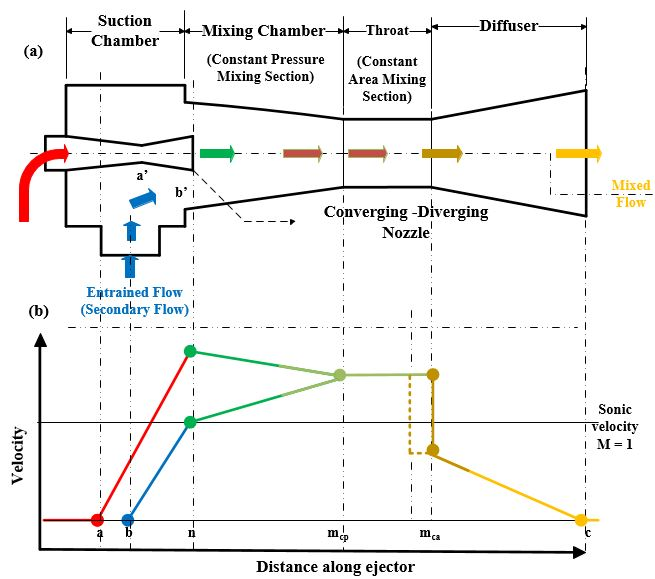
\includegraphics[height=4cm]{images/EjectorVelocityprofile.JPG}
    \caption{\scriptsize Velocity Profile versus distance along ejector}
    \end{figure}
\end{columns}
\end{frame}

\begin{frame}{Ejectors: Operating State Conditions}
    \begin{figure}[h]
    \centering
   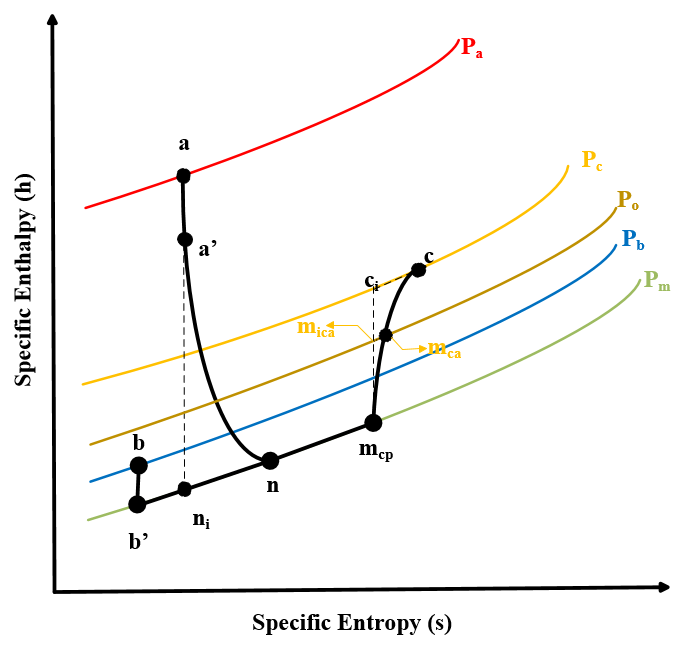
\includegraphics[height=4.5cm]{images/ejectorhsd.PNG}
    \caption{\scriptsize \centering Specific enthalpy (h) – Specific entropy (s) diagram of the processes inside the single-phase subsonic ejector}
    \label{fig:ejectorhsd}
\end{figure}
\end{frame}

\begin{frame}{Different types of ejector based on the location of the converging-diverging nozzle\cite{huang1985ejector}}
  \begin{columns}
    \column{0.45\textwidth}
    \begin{figure}[h]
      \centering
      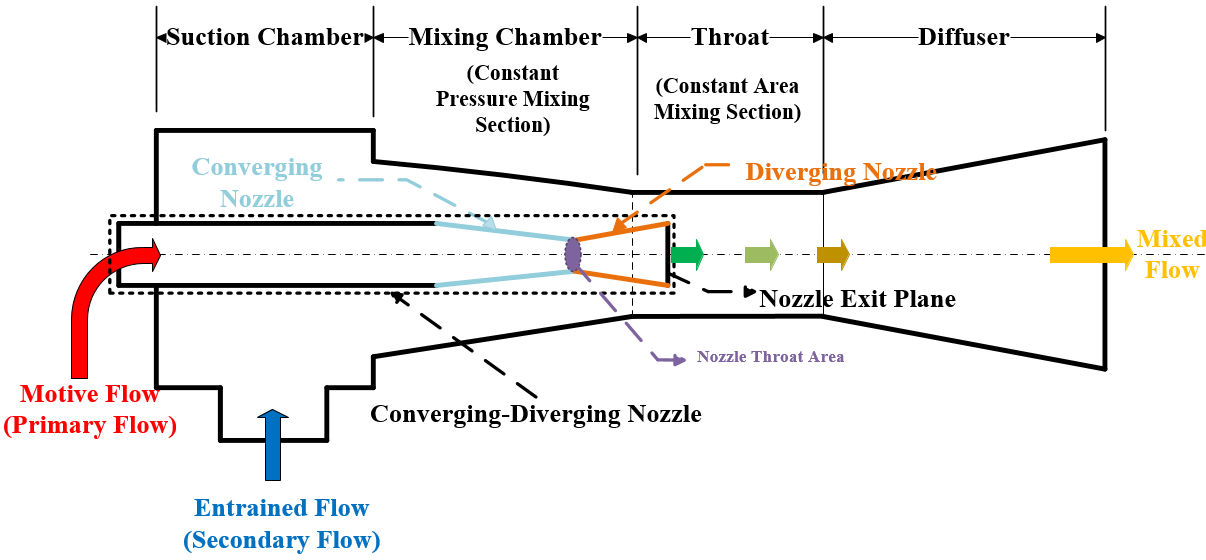
\includegraphics[height=2.5cm]{images/CAM ejector.PNG}
      \caption{CAM Ejector}
   \end{figure}
   \column{0.45\textwidth}
    \begin{figure}[h]
    \centering
    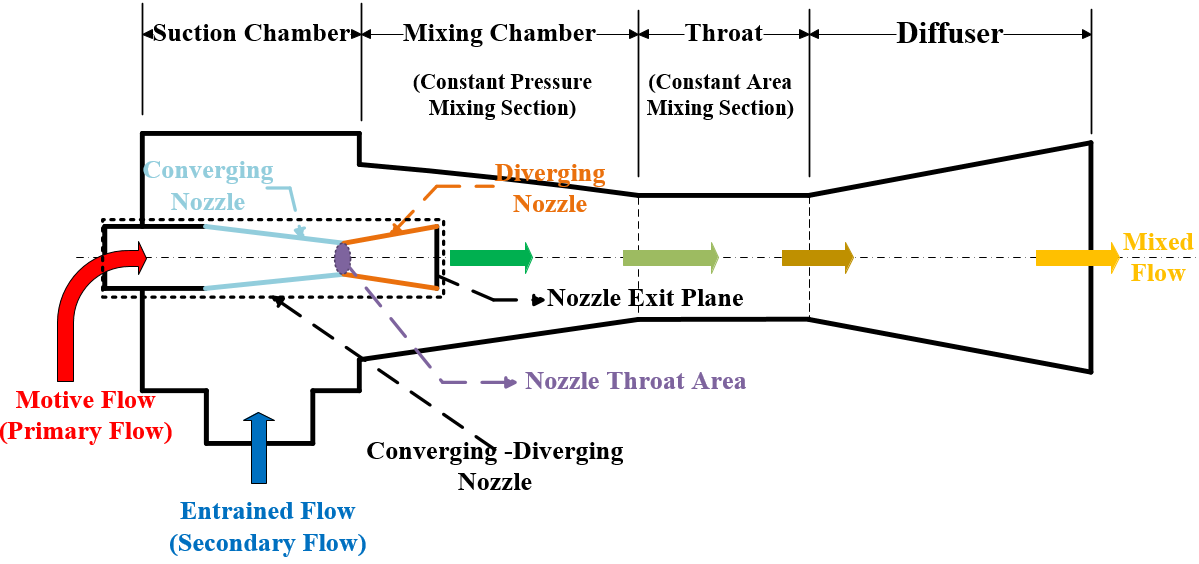
\includegraphics[height=2.5cm]{images/CPM ejector.PNG}
    \caption{CPM Ejector}
    \end{figure}
  \end{columns}
\end{frame}

\begin{frame}{Different Locations of Nozzle Exit Positions (NXP) of Ejector\cite{eames1999experimental,eames2007results,kumar2019effect,wang2017numerical, ramesh2018experimental, meyer2009steam}}
\begin{columns}
    \column{0.45\textwidth}
    \begin{figure}
        \centering
        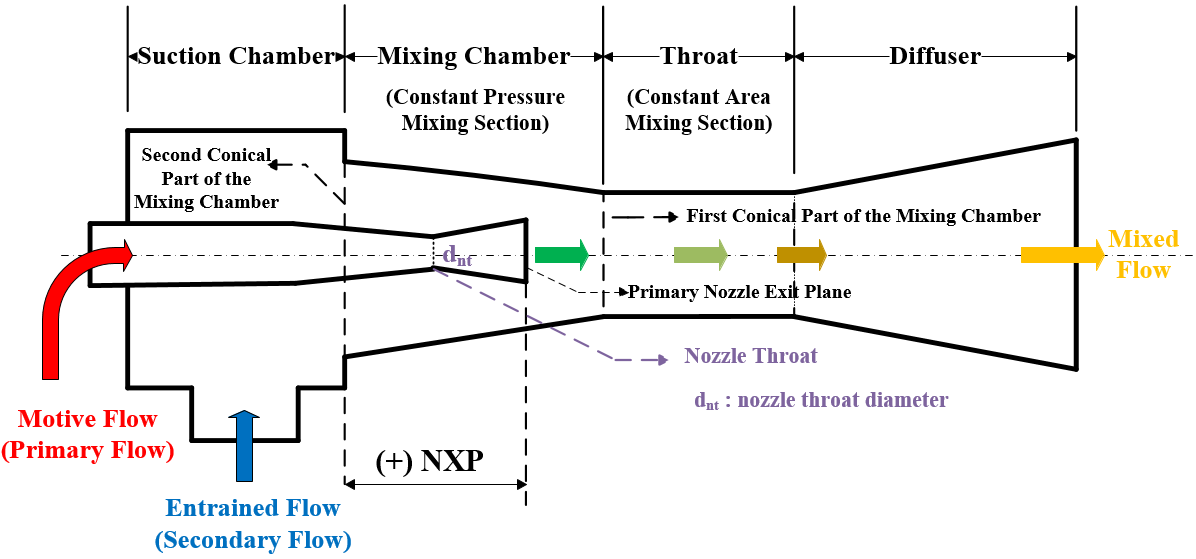
\includegraphics[height=2.5cm]{images/NXP+.PNG}
        \caption{\centering Positive NXP}
        \label{fig:nxppositive}
    \end{figure}
    \column{0.45\textwidth}
    \begin{figure}
        \centering
        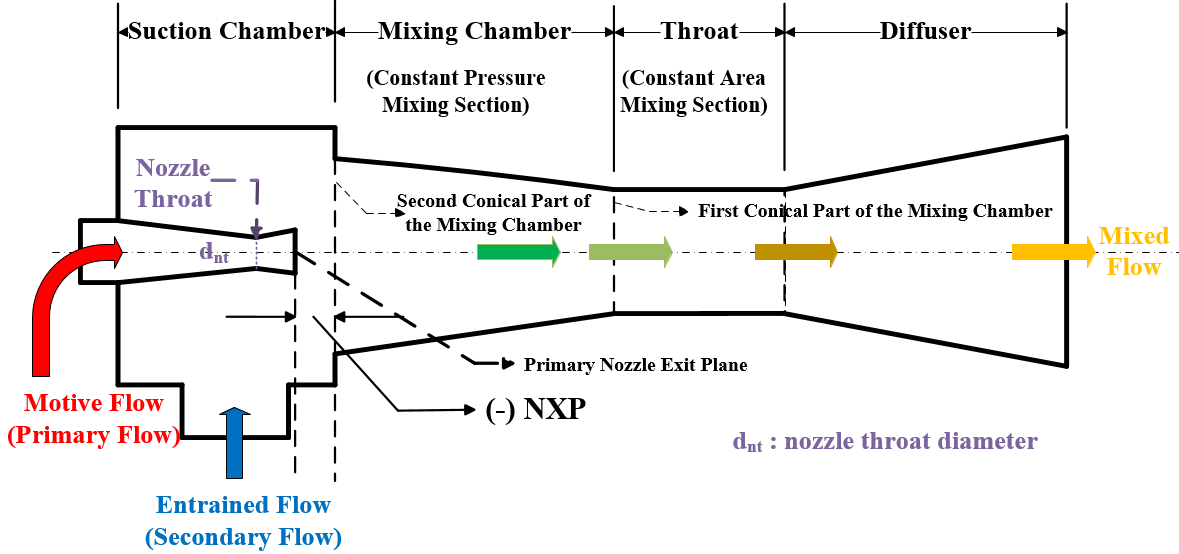
\includegraphics[height=2.5cm]{images/NXP-.PNG}
        \caption{\centering Negative NXP}
        \label{fig:nxpnegative}
    \end{figure}
\end{columns}
\end{frame}

\begin{frame}{Different Locations of Nozzle Exit Position (NXP) of Ejector\cite{eames1999experimental,eames2007results,kumar2019effect,wang2017numerical, ramesh2018experimental, meyer2009steam}}
    \begin{figure}
        \centering
        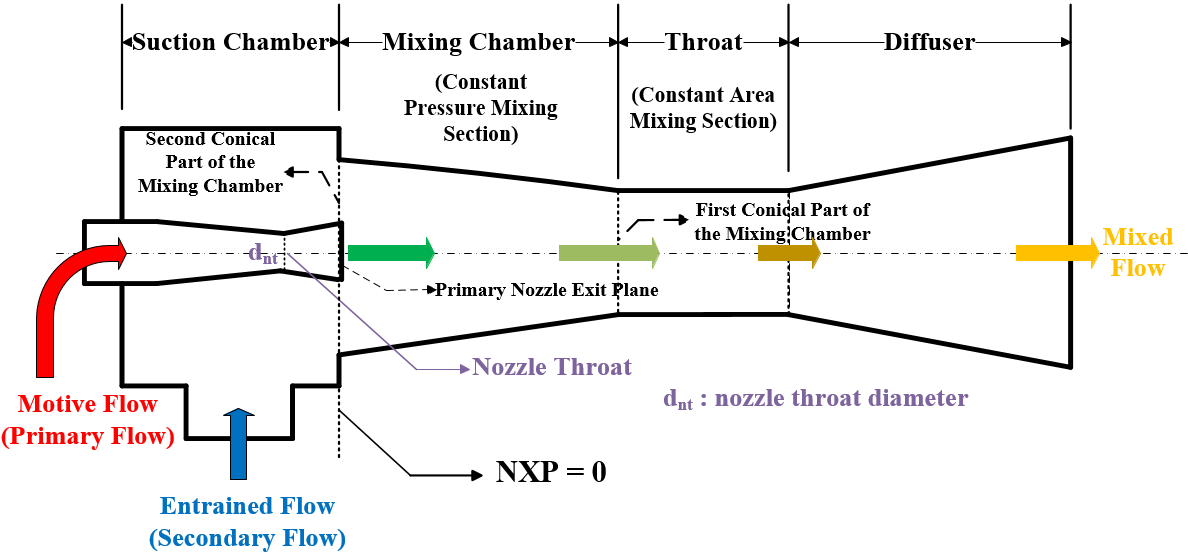
\includegraphics[height=3.5cm]{images/NXP0.PNG}
        \caption{\centering Zero NXP}
        \label{fig:nxpnxpzero}
    \end{figure}
\end{frame}

\begin{frame}{CAM and CPM Ejector: Review of Literature}
    Keenan et al. \cite{keenan1950investigation} proposed the concept of CPM ejector. Although CAM ejector can provide higher mass flow rates, the CPM ejectors are considered to be more favorable in practice for the merit of its stable performance at a wider range of backpressures \cite{tashtoush2019comprehensive}.
\end{frame}

\begin{frame}{Effect of NXP on the performance of the ejector\cite{tashtoush2019comprehensive}}
    \begin{table}[h]
        \centering
        \begin{tabular}{|p{2cm}|p{1.5cm}|p{4.5cm}|}
        \hline
            Model & Working Fluid & NXP\\
        \hline
             Experimental\cite{eames1999experimental} & Steam & Optimum (NXP/throat diameter) were found to vary in the range of -0.5 to 0.5 for a primary pressure ratio of 1.07 to 0.75, respectively \\
        \hline
             CFD and Experimental\cite{wang2018auto} & Methanol & Optimum NXP decreases as the primary flow pressure increases \\
        \hline
        \end{tabular}
    \end{table}
\end{frame}

\begin{frame}{Effect of NXP on the performance of the ejector\cite{tashtoush2019comprehensive}}
    \begin{table}[h]
        \centering
        \begin{tabular}{|p{2cm}|p{1.5cm}|p{5cm}|}
        \hline
            Model & Working Fluid & NXP\\
        \hline
             CFD and Experimental\cite{eames2007results} & R245fa & Optimum NXP is 5 mm upstream the entrance given entrainment ratio of 0.567, generator and evaporator temperatures of 120 and 12 $^{\circ}C$\\
        \hline
             Experimental\cite{meyer2009steam} & Steam & Optimum NXP is 5 mm upstream the entrance at boiler temperature of 85 to 110$^{\circ}C$ \\
        \hline
        \end{tabular}
    \end{table}
\end{frame}

\begin{frame}{Effect of NXP on the performance of the ejector\cite{tashtoush2019comprehensive}}
    \begin{table}[h]
        \centering
        \begin{tabular}{|p{2cm}|p{1.5cm}|p{4.5cm}|}
        \hline
            Model & Working Fluid & NXP\\
        \hline
             CFD \cite{varga2009influence} & Steam & Optimum NXP is 6 mm downstream the entrance\\
        \hline
             CFD\cite{zhu2009numerical} & R141a & Optimum (NXP/Diffuser throat diameter) is in the range of 1.7-3.4 upstream the entrance\\
        \hline
        \end{tabular}
    \end{table}
\end{frame}

\begin{frame}{Effect of NXP on the performance of the ejector\cite{tashtoush2019comprehensive}}
    \begin{table}[h]
        \centering
        \begin{tabular}{|p{2cm}|p{1.5cm}|p{5cm}|}
        \hline
            Model & Working Fluid & NXP\\
        \hline
             CFD \cite{yan2012geometry} & R134a & Optimum NXP is 8.91 mm upstream of the entrance\\
        \hline
             Experimental\cite{yapici2008experimental} & R123 & Among the tested ejectors it was found that optimum NXP values are always within -10 mm to 5 mm at which minimum suction pressure occurs in the suction chamber\\
        \hline
        \end{tabular}
    \end{table}
\end{frame}

\begin{frame}{Effect of NXP on the performance of the ejector\cite{tashtoush2019comprehensive}}
    \begin{table}[h]
        \centering
        \begin{tabular}{|p{2cm}|p{1.5cm}|p{5cm}|}
        \hline
            Model & Working Fluid & NXP\\
        \hline
             Experiment \cite{chunnanond2004ejectors} & Steam & Expansion waves of the jet core stream face stronger compression effect as NXP is moved upstream. Thus, a smaller expansion angle and a larger effective area would be produced\\
        \hline
             CFD\cite{hakkaki2015computational} & --- & Optimum NXP is 13 mm\\
        \hline
        \end{tabular}
    \end{table}
\end{frame}

\begin{frame}{Effect of NXP on the performance of the ejector\cite{tashtoush2019comprehensive}}
    \begin{table}[h]
        \centering
        \begin{tabular}{|p{2cm}|p{1.5cm}|p{5.5cm}|}
        \hline
            Model & Working Fluid & NXP\\
        \hline
             CFD \cite{omidvar2016entropy} & --- & Optimum NXP is 5 mm upstream corresponding to an improvement in performance of 37\% relative to the original geometry before optimization  \\
        \hline
             CFD\cite{chen2013numerical} & Natural gas & Maximum entrainment ratio is attained when the NXP is in the range of 3.6 to 7.2 mm. For optimum pressure ratio, NXP to be in the range of 1.2-7.2 mm\\
        \hline
        \end{tabular}
    \end{table}
\end{frame}

\begin{frame}{Effect of NXP on the performance of the ejector\cite{tashtoush2019comprehensive}}
    \begin{table}[h]
        \centering
        \begin{tabular}{|p{2cm}|p{1.5cm}|p{5cm}|}
        \hline
            Model & Working Fluid & NXP\\
        \hline
             Experiment\cite{jeon2017performance} & R600a for two-phase ejector & Maximum pressure lifting ratio was observed at NXP is 3 mm  \\
        \hline
             Numerical study\cite{pei2019numerical} & Hydrogen & The hydrogen entrainment ratio decreases dramaticallly in the whole operating range when NXP is above the optimal value range\\
        \hline
        \end{tabular}
    \end{table}
\end{frame}

\begin{frame}{Effect of NXP on the performance of the ejector\cite{tashtoush2019comprehensive}}
    \begin{table}[h]
        \centering
        \begin{tabular}{|p{2cm}|p{1.5cm}|p{5cm}|}
        \hline
            Model & Working Fluid & NXP\\
        \hline
             Experiment\cite{jeon2017performance} & R600a for two-phase ejector & Maximum pressure lifting ratio was observed at NXP is 3 mm  \\
        \hline
             Numerical study\cite{pei2019numerical} & Hydrogen & The hydrogen entrainment ratio decreases dramaticallly in the whole operating range when NXP is above the optimal value range\\
        \hline
        \end{tabular}
    \end{table}
\end{frame}

\begin{frame}{Effect of NXP on the performance of the ejector\cite{tashtoush2019comprehensive}}
    \begin{table}[h]
        \centering
        \begin{tabular}{|p{2cm}|p{1.5cm}|p{5cm}|}
        \hline
            Model & Working Fluid & NXP\\
        \hline
             Experiment and Numerical\cite{chong2014experimental} & --- & There exists an optimal NXP corresponding to maximum entrainment ratio, but the critical value of discharged pressure is almost independent of NXP  \\
        \hline
        \end{tabular}
    \end{table}
\end{frame}

\begin{frame}{Applications of Commercially Available Steam Ejector\cite{SchutteandKoerting}}
  \begin{columns}
    \column{0.45\textwidth}
    \begin{itemize}
        \item Supplying heated water to jackets of stills and graining bowls
        \item Intermittent pumping of liquids from tanks and pits
        \item Condensing and mixing ammonia
        \item Pipeline heater
        \item Pumping waste water from quench tanks and cleaning inline pipes with heated water in steel processing
    \end{itemize}
    \column{0.45\textwidth}
    \begin{figure}
        \centering
        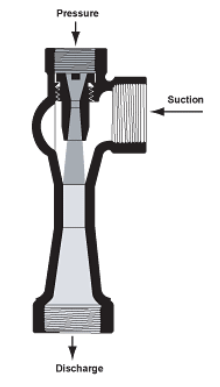
\includegraphics[height=4.5cm]{images/schutteandkoertingthermosyphon.png}
        \caption{\centering Steam Jet Syphon(Commercially Available Steam Ejectors) photo courtesy of Schutte and Koerting \cite{SchutteandKoerting}}
    \end{figure}
  \end{columns}
\end{frame}

\begin{frame}{Applications of Commercially Available Steam Ejector\cite{SchutteandKoerting}}
  \begin{columns}
    \column{0.45\textwidth}
    \begin{itemize}
        \item Used on dust collecting equipment
        \item Used for draining large receptacles of waste process
        \item Condensing and mixing ammonia
        \item Automatic pumping of chemical spill
        \item Automatic pumping of condensate sump for power industry
    \end{itemize}
    \column{0.45\textwidth}
    \begin{figure}
        \centering
        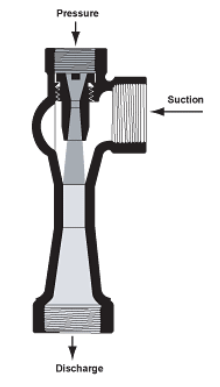
\includegraphics[height=4.5cm]{images/schutteandkoertingthermosyphon.png}
        \caption{\centering Steam Jet Syphon(Commercially Available Steam Ejectors) photo courtesy of Schutte and Koerting \cite{SchutteandKoerting}}
    \end{figure}
  \end{columns}
\end{frame}

\begin{frame}{Applications of Commercially Available Steam Ejector\cite{SchutteandKoerting}}
  \begin{columns}
    \column{0.45\textwidth}
    \begin{itemize}
        \item Automatic pumping of water in hot house in agricultural industry
        \item Pumping filtrate from vacuum vessels and condensate from surface condensers
        \item Supplying heated water to the jackets of stills and graining bowls
        \item Removing liquid from pickling baths.
        \item Extracting chemicals in reaction chambers
    \end{itemize}
    \column{0.45\textwidth}
    \begin{figure}
        \centering
        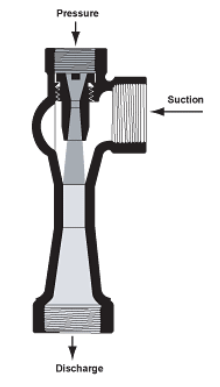
\includegraphics[height=4.5cm]{images/schutteandkoertingthermosyphon.png}
        \caption{\centering Steam Jet Syphon (Commercially Available Steam Ejectors) photo courtesy of Schutte and Koerting \cite{SchutteandKoerting}}
    \end{figure}
  \end{columns}
\end{frame}

\begin{frame}{Applications of Commercially Available Steam Ejector\cite{SchutteandKoerting}}
  \begin{columns}
    \column{0.45\textwidth}
    \begin{itemize}
        \item Moving powdered material or material in granular form
        \item Filling and emptying gas holder tanks
        \item Handling soap solutions in textile plants
        \item Pumping sugar juice and various liquids in canning plants
    \end{itemize}
    \column{0.45\textwidth}
    \begin{figure}
        \centering
        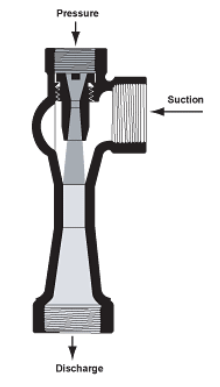
\includegraphics[height=4.5cm]{images/schutteandkoertingthermosyphon.png}
        \caption{\centering Steam Jet Syphon (Commercially Available Steam Ejectors) photo courtesy of Schutte and Koerting \cite{SchutteandKoerting}}
    \end{figure}
  \end{columns}
\end{frame}

\begin{frame}{Commercially Available Steam Ejectors: Steam Jet Syphons\cite{SchutteandKoerting}}
    \begin{table}[h]
    \centering
    \caption{\centering \scriptsize Different Sizes of Steam Jet Syphons based from the Ejector Manufacturer Schutte \& Koerting\cite{SchutteandKoerting}}
    \label{tab:SteamJetSyphons_workingpress}
    \begin{tabular}{|c|c|c|c|c|c|c|}
    \hline
        Size & \multicolumn{3}{c|}{Steam Inlet Pressure (kPa)} & \multicolumn{3}{c|}{Liquid Inlet Pressure (kPa)}\\
    \cline{2-7}
        No. & Cast Iron & Bronze & Stainless Steel & Cast Iron & Bronze & Stainless Steel \\
    \hline
        1 & 1207 & 862 & 3450 & 862 & 690 & 2070 \\
    \hline
        2 & 1207 & 862 & 3450 & 862 & 690 & 2070 \\
    \hline
        3 & 1207 & 862 & 3450 & 862 & 690 & 2070 \\
    \hline
        4 & 1035 & 862 & 3450 & 690 & 690 & 2070 \\
    \hline
        5 & 1035 & 862 & 3450 & 690 & 690 & 2070 \\
    \hline
        6 & 1380 & 1380 & 3450 & 690 & 690 & 2070 \\
    \hline
        \textbf{7} & 1380 & 1380 & \textbf{3450} & 690 & 690 & \textbf{2070} \\
    \hline
        8\textsuperscript{a} & 862 & --- & --- & 862 & --- & --- \\
    \hline
        9\textsuperscript{a} & 862 & --- & --- & 862 & --- & --- \\
    \hline
    \end{tabular}
\end{table}
\end{frame}

\begin{frame}{Dimensions of Different Sizes of Steam Jet Syphons based from the Ejector Manufacturer Schutte \& Koerting\cite{SchutteandKoerting}}
\begin{columns}
    \column{0.45\textwidth}
       \begin{table}[h]
       \label{tab:SteamJetSyphons_sizes}
       \begin{tabular}{|c|c|c|c|}
        \hline
        Size & \multicolumn{3}{c|}{Dimensions (mm)}  \\
        \cline{2-4}
        No & A & B & C \\
        \hline
        1 & 27 & 65 & 29 \\
        \hline
        2 & 35 & 86 & 32 \\
        \hline
        3 & 38 & 110 & 41 \\
        \hline
        4 & 51 & 165 & 51 \\
       \hline
        5 & 57 & 194 & 57 \\
       \hline
        6 & 68 & 235 & 79 \\
       \hline
        \textbf{7} & \textbf{80} & \textbf{286} & \textbf{89} \\
        \hline
        8 & 112 & 490 & 198 \\
        \hline
        9 & 155 & 721 & 232 \\
        \hline
        \end{tabular}
       \end{table}
   \column{0.35\textwidth}
    \begin{figure}[h]
    \centering
    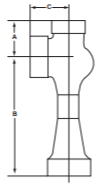
\includegraphics[height=5cm]{images/Syphonsshcutteandkoerting.PNG}
    \end{figure}
  \end{columns}
\end{frame}

\begin{frame}{Steam Jet Vacuum Systems\cite{NASH:Technology}}
    \begin{columns}
    \column{0.45\textwidth}
       \begin{itemize}
           \item \small Uses High-Pressure High-Temperature steam as a motive fluid to entrain the pressurized water in the steam ejector
           \item \small High-pressure high-temperature steam inflowing to the converging-diverging nozzle flushes the non-condensible gases inside the ejector, thus, making it a vacuum system.
           \item \small Steam jet vacuum system is used in large-scale thermal power plants (i.e. large power capacity geothermal power plants), thus making it beyond the scope of this study.
       \end{itemize}
   \column{0.45\textwidth}
    \begin{figure}[h]
    \centering
    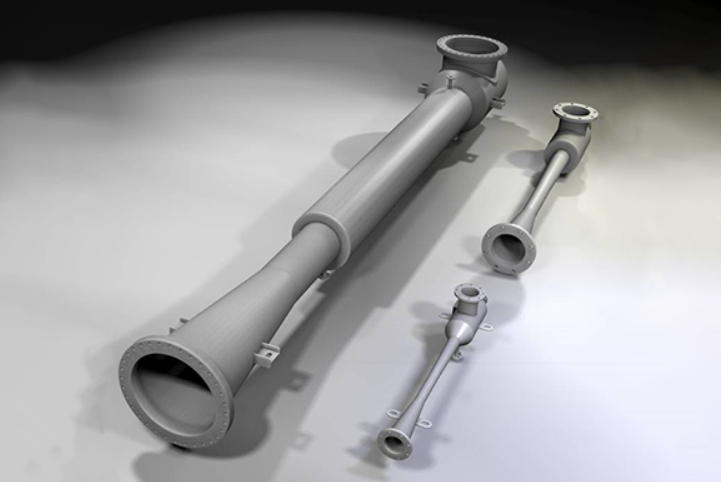
\includegraphics[height=4cm]{images/SteamVacuumsystem.PNG}
    \caption{Photo courtesy of Gardner Denver\cite{NASH:Technology}}
    \end{figure}
  \end{columns}
\end{frame}

\begin{frame}{\small Novel Open Hybrid Trilateral Flash Partial Evaporating Cycle Geothermal Power Plant Incorporated in an Ejector(NOHTFPECGPPIE)}
    \begin{columns}
    \column{0.45\textwidth}
    \begin{figure}[h]
      \centering
      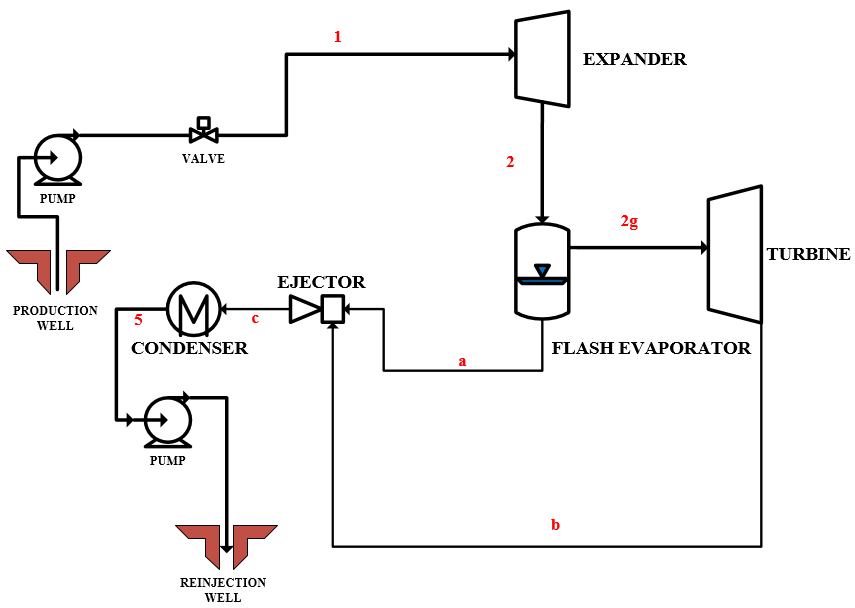
\includegraphics[height=3.5cm]{images/NOHTFPECGPPIE.PNG}
      \caption{\scriptsize \centering Schematic Diagram of the NOHTFPECGPPIE}
      \label{fig:nohtfpecgppieschematicdiagram}
   \end{figure}
   \column{0.45\textwidth}
    \begin{figure}[h]
    \centering
    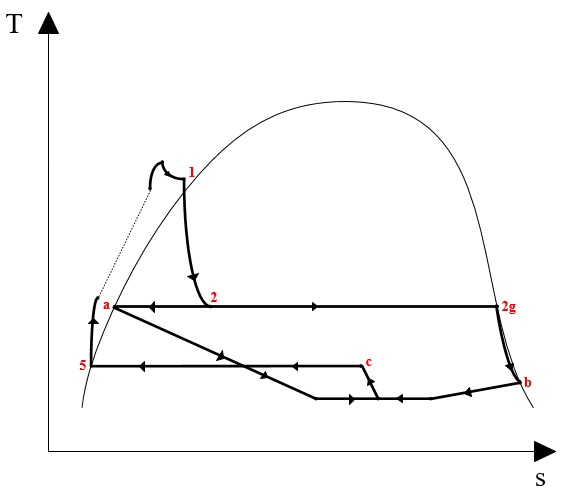
\includegraphics[height=3.75cm]{images/nohtfpecgppietsdiagram.jpg}
    \caption{\scriptsize \centering Temperature (T) versus specific entropy (s) diagram of NOHTFPECGPPIE}
    \label{fig:nohtfpecgppietsdiagram}
    \end{figure}
\end{columns}
\end{frame}

\begin{frame}{Problem Statement}
  \begin{block}{Ideal Situation}
   NOHTFPECGPPIE operates on a driven central water jet steam ejector low-enthalpy-to-power conversion cycle.
  \end{block}
  \begin{block}{Actual Situation}
   \begin{itemize}
       \item Majority of the ejector (especially steam ejector) applies to refrigeration system and less in the power generation systems.
       \item  Majority of the steam ejector in operates on single phase flows and less in two-phase flows.
       \item Two-phase flow steam ejector is flowing at supersonic state uses steam as a motive fluid enough to entrain the liquid water
   \end{itemize}
  \end{block}
\end{frame}

\begin{frame}{Problem Objectives}
    In able to prepare the proposed NOHTFPECGPPIE to execute on a test scale, the following objective must be attained:
   \begin{itemize}
    \item Validate the CFD model of the replicated subsonic steam central core driven ejector design (e.g. SJP3) from the existing experimental data and ejector design of Shah et al. \cite{shah2014experimental} thru ANSYS Fluent R18 software.
    \item After validation, reverse the flow in the steam ejector by using pressurized water as a motive fluid and steam as an entrained fluid and simulate the CFD model using ANSYS Fluent R18 software.
  \end{itemize}
\end{frame}

\begin{frame}{Problem Objectives}
    \begin{itemize}
        \item Investigate the use of a brine as a working fluid replacing of pure water in the steam ejector.The brine properties and geothermal well head pressure are obtained from the slimhole of Tingloy Geothermal Power Plant from the Department of Energy.
        \item Conduct sensitivity analysis in the ejector by conducting a partial evaporation on the pressurized water in the ejector with respect to the given ejector geometries and operating conditions.
       \item Compare the NOHTFPECGPPIE to other power generation cycles that uses low-grade thermal or low-enthalpy as a source of heat energy.
    \end{itemize}
\end{frame}

\begin{frame}{Significance of the Problem}
    The study about the CFD model of the ejector of NOHTFPECGPPIE will provide feasibility for the possible laboratory test scale of NOHTFPECGPPIE. This study will also fill the following research gaps, namely as follows:
  \begin{enumerate}
    \item Flow Mechanism of a Subsonic Water Central Jet Driven Two-phase flow steam ejector
    \item Trilateral Flash Cycles, 
    \item Partial Evaporation Technique for Low-Temperature-to-Power Conversion Cycles, and 
    \item The use of the ejector for power recovery low-enthalpy power generating cycles.
  \end{enumerate}
\end{frame}

\begin{frame}{Scope and Limitation of the Study}
The scope of this study is based on the numerical modelling thru ANSYS Fluent. The numerical models are as follows, namely:
   \begin{itemize}
       \item Eulerian Multiphase Models
           \begin{itemize}
               \item Two-Resistance Heat Transfer Model
               \item Thermal Phase Change Model
               \item Explicit Model
           \end{itemize}
       \item $\kappa-\varepsilon$ realizable per phase turbulence models
           \begin{itemize}
               \item Scalable Wall Function
           \end{itemize}
   \end{itemize}
\end{frame}

\begin{frame}{Eulerian Multiphase Model: Limitation of the Model}
    The Eulerian multiphase models has the following limitation, namely:
\begin{enumerate}
    \item Reynolds Stress turbulence model is not available on a per phase basis
    \item Particle tracking (using the Lagrangian dispersed phase model) interacts only with the primary phase
    \item Streamwise periodic flow with specified mass flow rate cannot be modeled, however, specification of a pressure drop is allowed.
    \item Inviscid flow is not allowed.
    \item Melting and solidification are not allowed.
    \item When tracking particles in parallel, the DPM model cannot be used with the Eulerian multiphase model if the shared memory option is enabled. This operation is in relation to the Parallel Processing for the Discrete Phase Model in the ANSYS User’s Guide. 
\end{enumerate}
\end{frame}

\begin{frame}{Limitation and Features: $\kappa-\varepsilon$ realizable turbulence models}
   \begin{itemize}
       \item Limits its use in non-multiple reference frames and non-rotating sliding meshes because it produces non-physical turbulent viscosities(i.e. extra rotational effects) in moving reference frames.
       \item Addresses the weaknesses of a standard $\kappa-\varepsilon$ or other traditional $\kappa-\varepsilon$ in well-known round-jet anomaly. The round-jet anomaly is the flow-spreading rate in planar or axisymmetric jets.
       \item Realizable $\kappa-\varepsilon$ gives better prediction than standard $\kappa-\varepsilon$  in spreading rates in planar and axisymmetric jets by introducing a new model equation for the dissipation ($\varepsilon$).
   \end{itemize}
\end{frame}

\begin{frame}{Per Phase Turbulence Model: Features of the Model}
\begin{itemize}
    \item Per Phase treatment of Realizable $\kappa-\varepsilon$ turbulence model in this study is the most general multiphase turbulence model that solves a set of $\kappa$ and $\varepsilon$ transport equations for each phase.
    \item Limits of this turbulence model applies to the either phases playing a dominant role in turbulence transfer like condensation and evaporation phenomena between two phases (e.g. steam and water phases).
\end{itemize}
\end{frame}